%        File: hw1.tex
%     Created: Sat Apr 06 10:00 AM 2013 P
% Last Change: Sat Apr 06 10:00 AM 2013 P
%
\documentclass[11pt]{article}

\usepackage{amsmath, amssymb, amsthm, cite, graphicx, float, mathrsfs, commath, dsfont, bbm, bm}
\usepackage[mathscr]{eucal}
\usepackage[sc]{mathpazo}
\linespread{1.05}
%\usepackage{setspace}
%\onehalfspacing
\usepackage[margin=1in, top=.8in, left=.8in]{geometry}
\usepackage{color}

% new commands
\DeclareMathOperator*{\argmin}{arg\,min}
\DeclareMathOperator{\sgn}{sgn}
\newcommand{\E}{\mathrm{E}}
\newcommand{\Var}{\mathrm{Var}}
\newcommand{\Cov}{\mathrm{Cov}}
\newcommand{\Cor}{\mathrm{Cor}}
\newcommand{\id}{\operatorname{id}}
\newcommand{\diag}{\operatorname{diag}}
\newcommand{\Id}{\operatorname{Id}}
\newcommand{\tr}{\operatorname{tr}}
\newcommand{\Q}{\mathbb{Q}}
\newcommand{\C}{\mathbb{C}}
\newcommand{\R}{\mathbb{R}}
\newcommand{\Z}{\mathbb{Z}}
\newcommand{\F}{\mathbb{F}}
\newcommand{\N}{\mathbb{N}}

\newcommand{\indep}{\rotatebox[origin=c]{90}{$\models$}}

% 524 commands
%\newcommand{\norm}[1]{\| #1 \|}
\DeclareMathOperator{\spn}{span}
%\newcommand{\spn}{\operatorname{span}}
\newcommand{\onenorm}[1]{\| #1 \|_{L^1(\mathbb R^d)}}
\newcommand{\twonorm}[1]{\| #1 \|_{L^2(\mathbb R^d)}}

% 534 commands
\renewcommand{\Re}{\text{Re\,}}
\renewcommand{\Im}{\text{Im\,}}

\begin{document}
\pagestyle{empty}
\hfill Abraham Engle

\hfill Stat 571

\hfill \today
\begin{enumerate}
    %1
	\item In the last homework we had two working covariance matrix assumptions, AR(1) and Exchangeable. I first include plots of the dental data that were presented in the first chapter using spaghetti plots and conditional plots:
	\begin{figure}[H]
		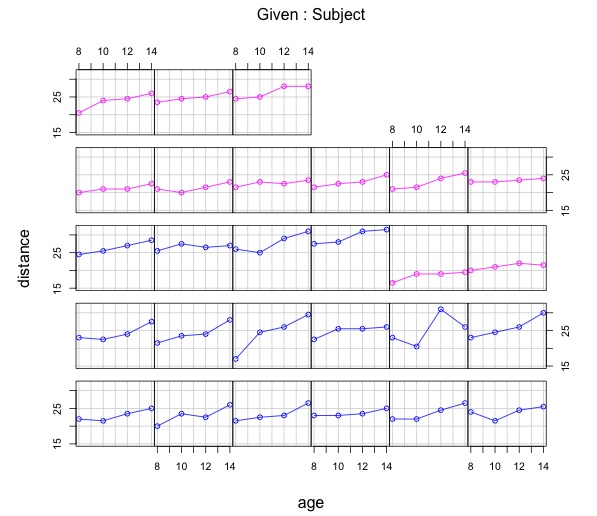
\includegraphics[scale=0.4]{RplotConditional.png}
		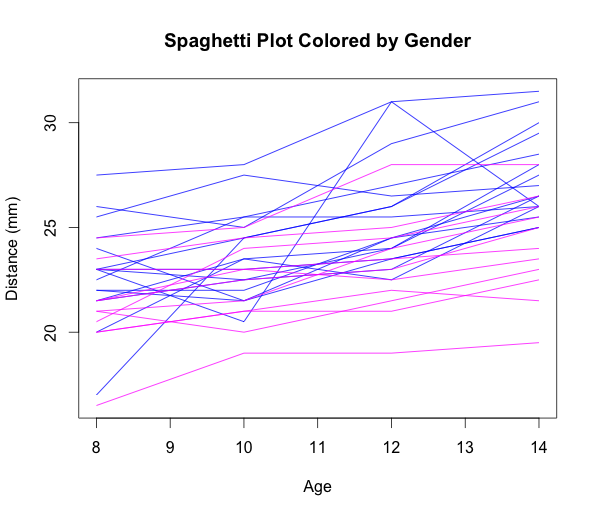
\includegraphics[scale=0.4]{RplotSpaghetti.png}
	\end{figure}
 	The ninth male subject with the oscillating distances catches my eye like we mentioned in class, and I'll keep that individual in mind when looking at diagnostics later. I next examined whether the empirical distribution of $\widehat{\bm{\beta}}$ looks approximately normal under both working correlation assumptions using the bootstrap method with $B=1000$ samples.
		\begin{figure}[H]
			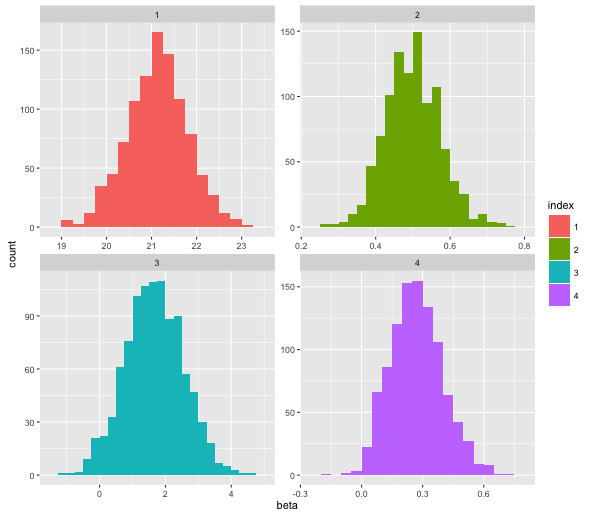
\includegraphics[scale=0.4]{RplotFirstBoot_AR1}
			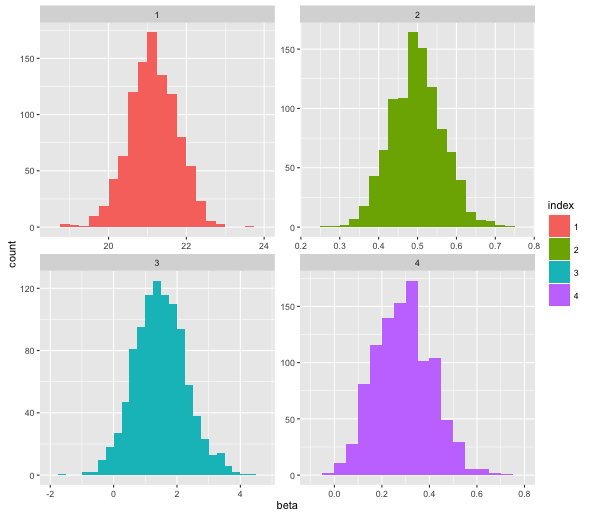
\includegraphics[scale=0.4]{RplotFirstBoot_Exch}
		\end{figure}
		The graphs do not raise any concerns to me. I next performed leave one out diagnostics both based on bootstrap and from GEE (which was much quicker) like discussed in class, beginning with AR(1):
		\begin{figure}[H]
			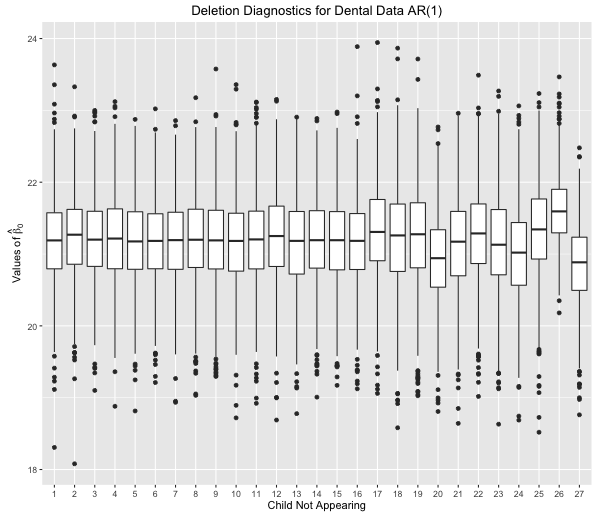
\includegraphics[scale=0.4]{RplotDDAR1Beta0.png}
			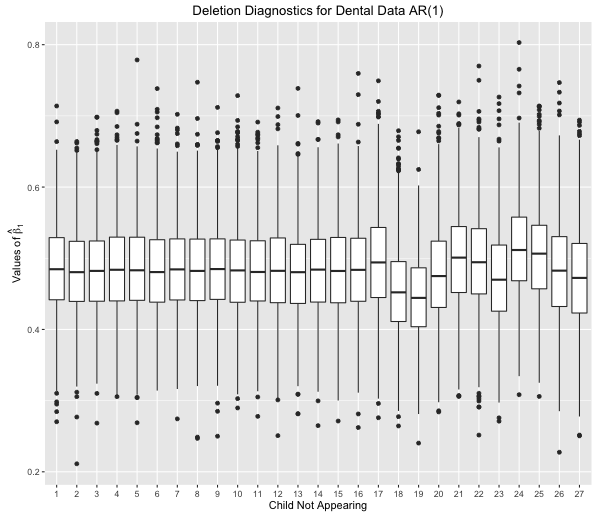
\includegraphics[scale=0.4]{RplotDDAR1Beta1.png}
			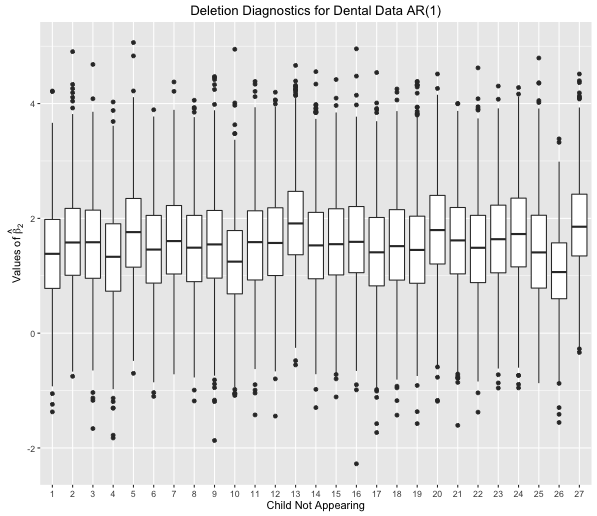
\includegraphics[scale=0.4]{RplotDDAR1Beta2.png}
			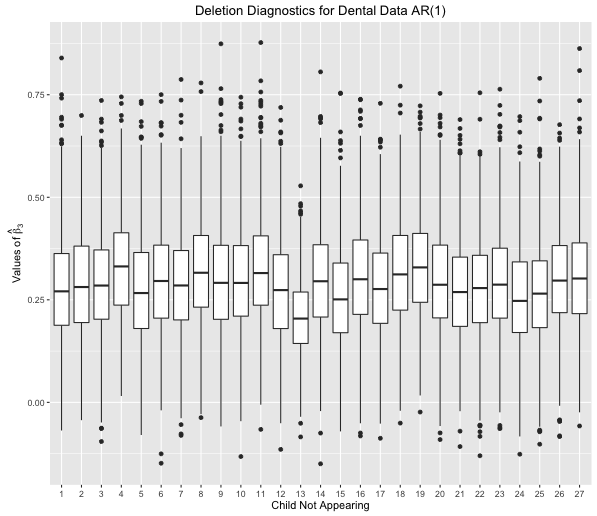
\includegraphics[scale=0.4]{RplotDDAR1Beta3.png}
		\end{figure}
		and GEE:
		\begin{figure}[H]
			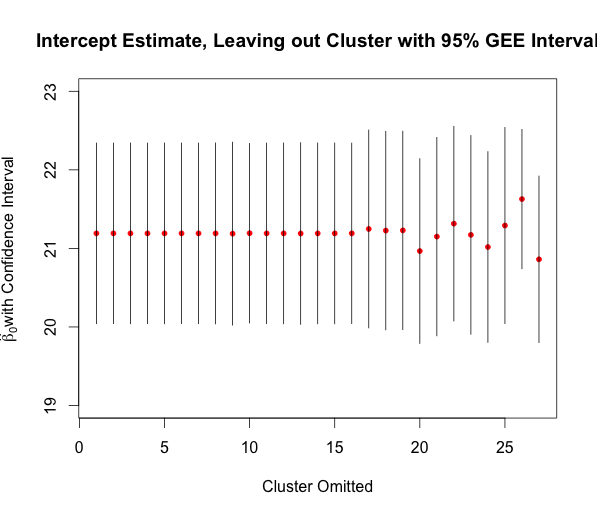
\includegraphics[scale=0.4]{RplotDDAR1GEEBeta0.png}
			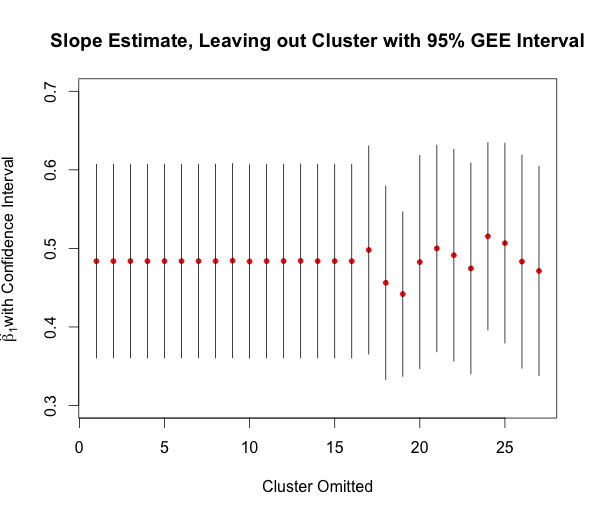
\includegraphics[scale=0.4]{RplotDDAR1GEEBeta1.png}
			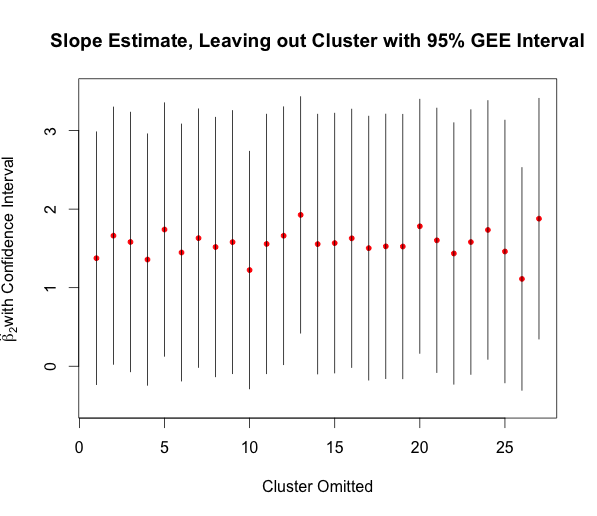
\includegraphics[scale=0.4]{RplotDDAR1GEEBeta2.png}
			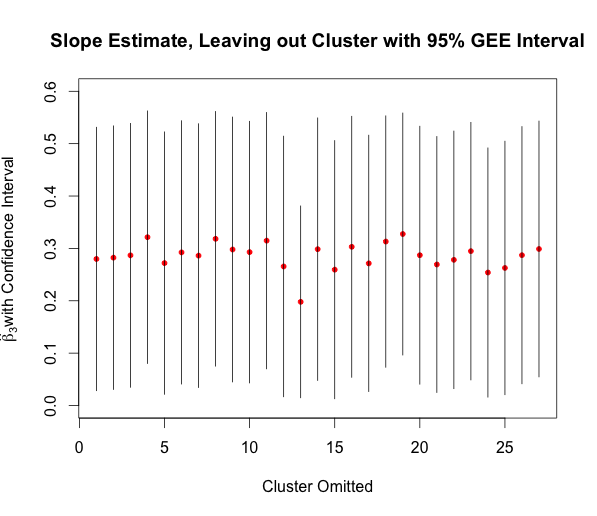
\includegraphics[scale=0.4]{RplotDDAR1GEEBeta3.png}	
		\end{figure}
		We noticed in class with the measles data and on the last homework set that point estimates do not change very much when changing working correlations, so I should not expect these plots to look too different when switching to an exchangeable correlation matrix. The bootstrap boxplots are:
		\begin{figure}[H]
			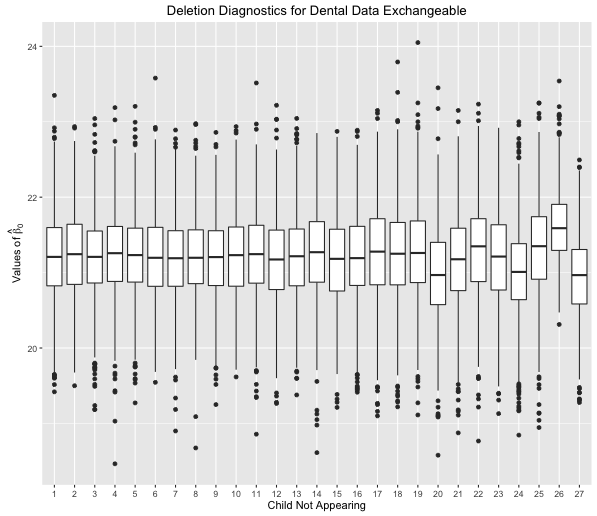
\includegraphics[scale=0.4]{RplotDDExchBeta0.png}
			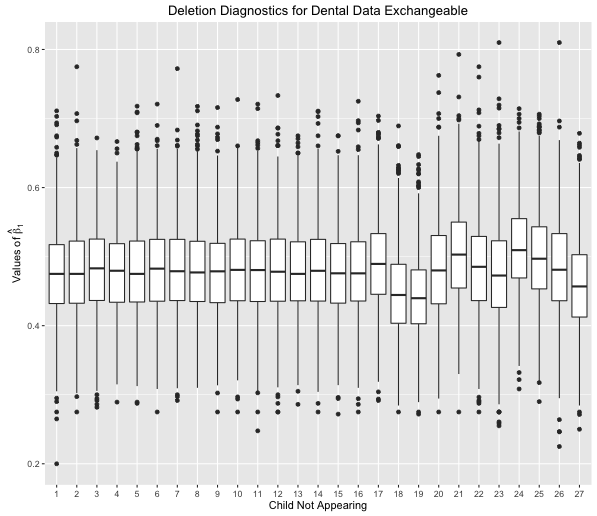
\includegraphics[scale=0.4]{RplotDDExchBeta1.png}
			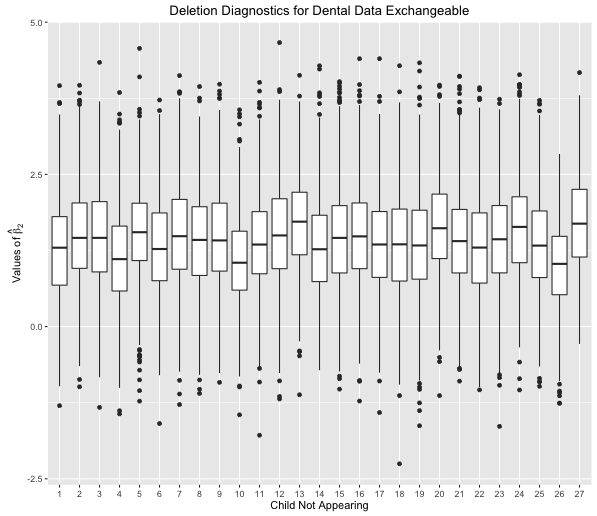
\includegraphics[scale=0.4]{RplotDDExchBeta2.png}
			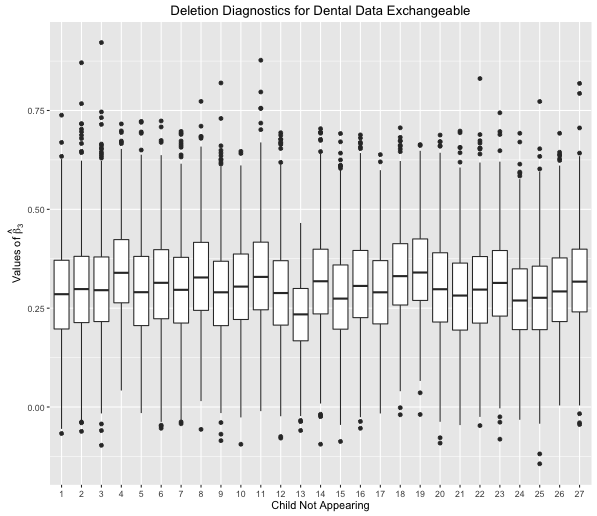
\includegraphics[scale=0.4]{RplotDDExchBeta3.png}
		\end{figure}
		and from GEE:
		\begin{figure}[H]
			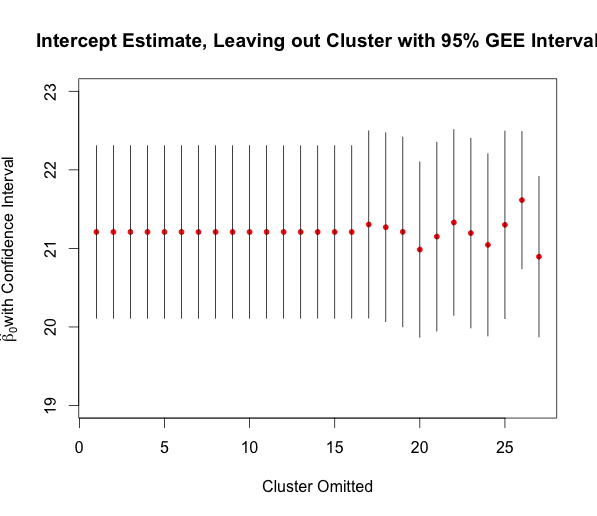
\includegraphics[scale=0.4]{RplotDDExchGEEBeta0.png}
			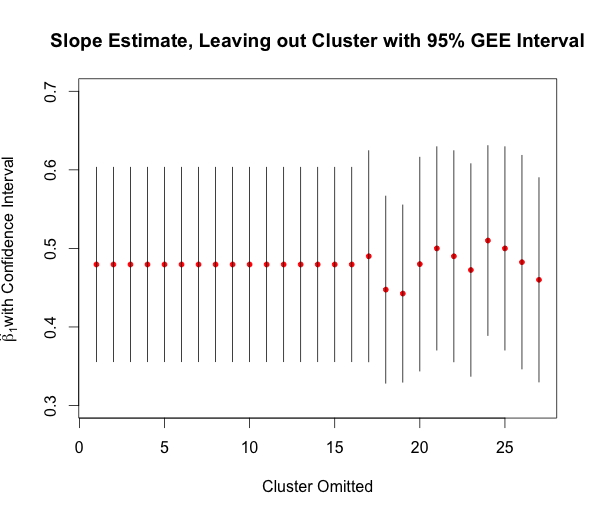
\includegraphics[scale=0.4]{RplotDDExchGEEBeta1.png}
			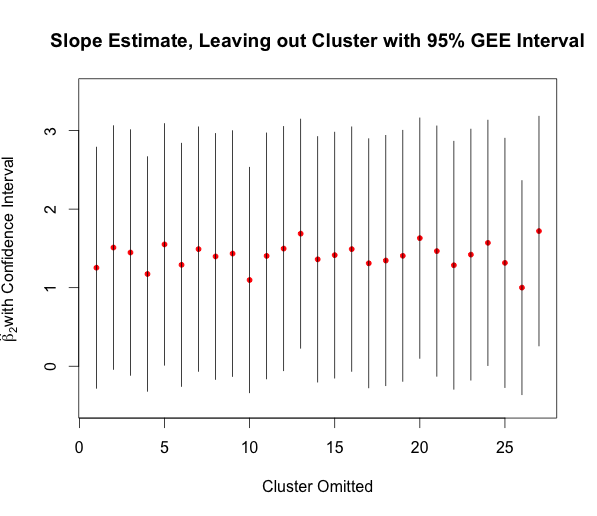
\includegraphics[scale=0.4]{RplotDDExchGEEBeta2.png}
			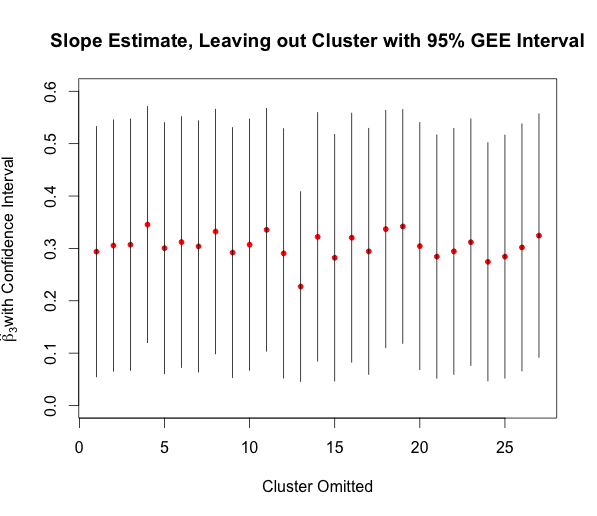
\includegraphics[scale=0.4]{RplotDDExchGEEBeta3.png}	
		\end{figure}
		Keeping in mind that some data point necessarily looks worst and that we're focusing on the intercept, I am going to look a bit closer at clusters 13 and 19 (male 13 and female 3). I do, however, think $n=27$ is big enough so that asymptotic approximations to the distribution of $\widehat\beta$ work well. I plot the Pearson residuals against fitted values (which should have mean zero at all fitted values) and against cluster index (for closer examination of male 13 and female 3) for both working correlation assumptions.
		\begin{figure}[H]
			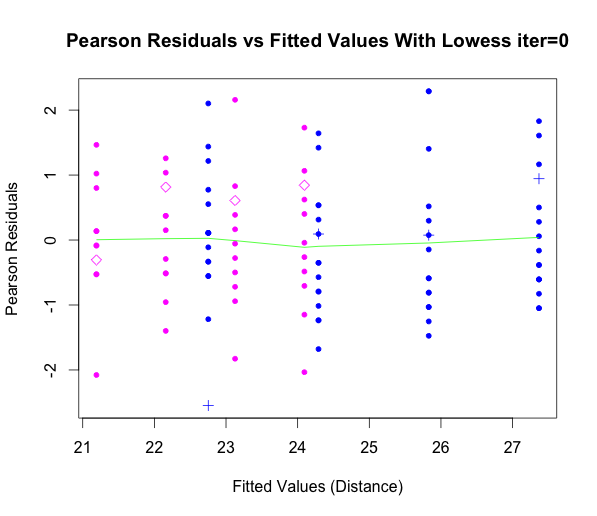
\includegraphics[scale=0.4]{RplotAR1Mean1}
			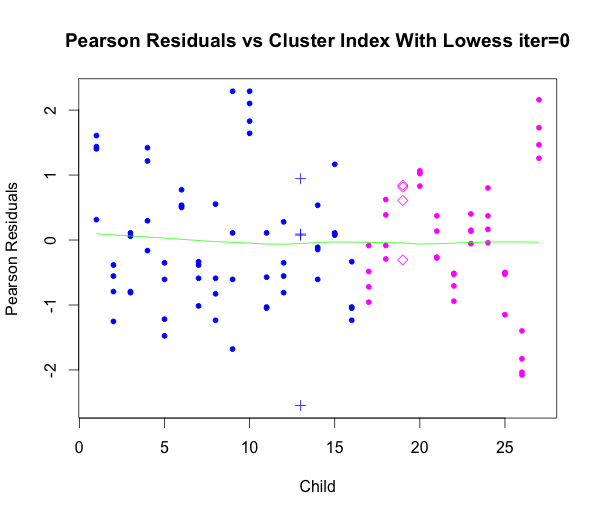
\includegraphics[scale=0.4]{RplotAR1Mean2}
			\caption{Mean Model Diagnostics Under AR(1) Assumption. + is Male 13, Diamond is Female 3}
		\end{figure}

		\begin{figure}[H]
			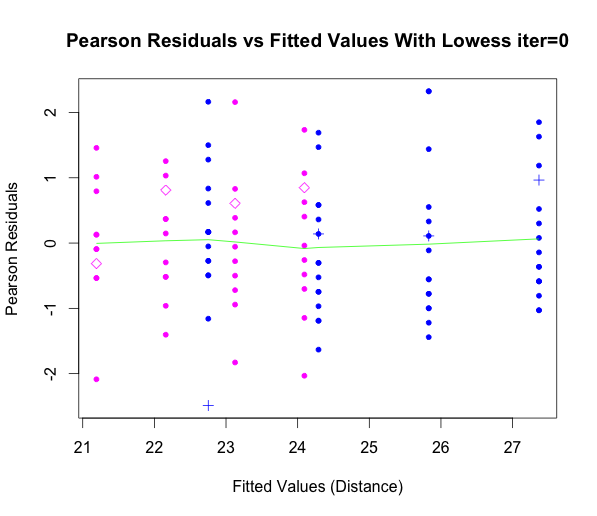
\includegraphics[scale=0.4]{RplotExchMean1}
			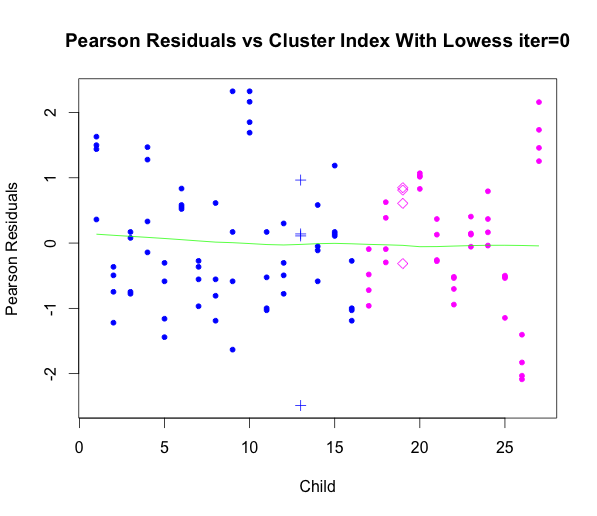
\includegraphics[scale=0.4]{RplotExchMean2}	
			\caption{Mean Model Diagnostics Under Exchangeable Assumption. + is Male 13, Diamond is Female 3}
		\end{figure}
		I think the fitted mean looks good in all four plots. If the variance assumption is additionally correct, the squared residuals should have mean 1 everywhere:
		\begin{figure}[H]
			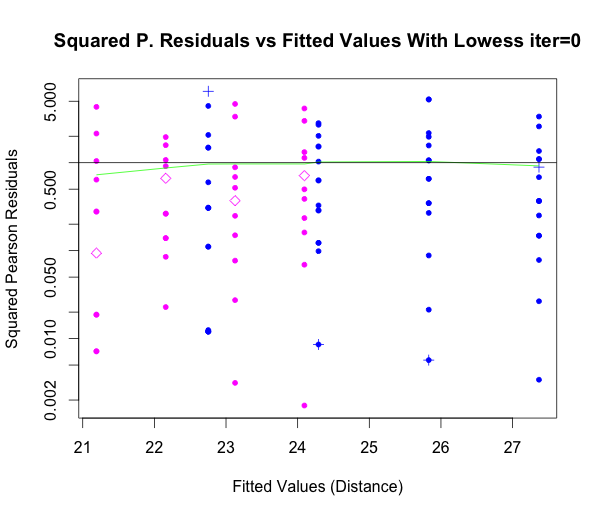
\includegraphics[scale=0.4]{RplotAR1Var.png}	
			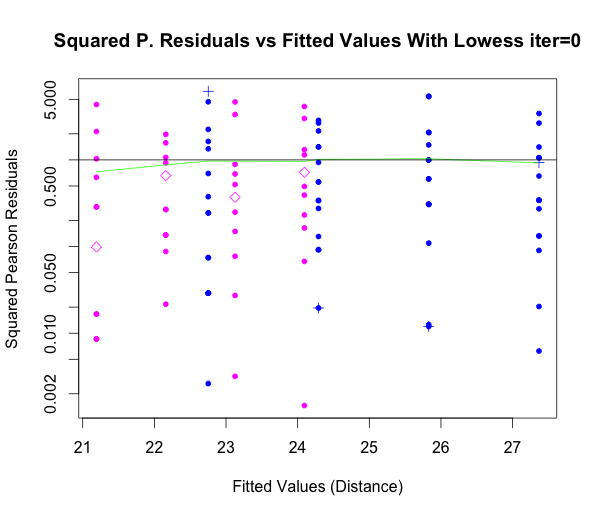
\includegraphics[scale=0.4]{RplotExchVar.png}
			\caption{Variance Diagnostics (Logarithmic y-axis). Left: AR(1) Right: Exchangeable. + is Male 13, Diamond is Female 3}
		\end{figure}
		Like the slides say, violations of this assumption only affect efficiency, but I believe the plots do not suggest huge violation. To be fair, there do seem to be more points lying below 1 than above. The smoother passes through mean 1 almost perfectly in both plots, however. The female cluster's residuals do not appear out of the ordinary in any of the above plots. Male 13 has the most negative residual in the entire batch, and examining the coplot at the start, it looks like that subject has the smallest distance at age 8 in the entire group of kids, so it looks like that child has high leverage. Addressing the child whose distances oscillated strangely (cluster 9), I did not really notice that cluster in the leave-one-out diagnostics nor did that cluster come up in the examining the residuals. I finally tried plotting a semivariogram for the AR(1) working correlation assumption:
		\begin{figure}[H]
			\centering
			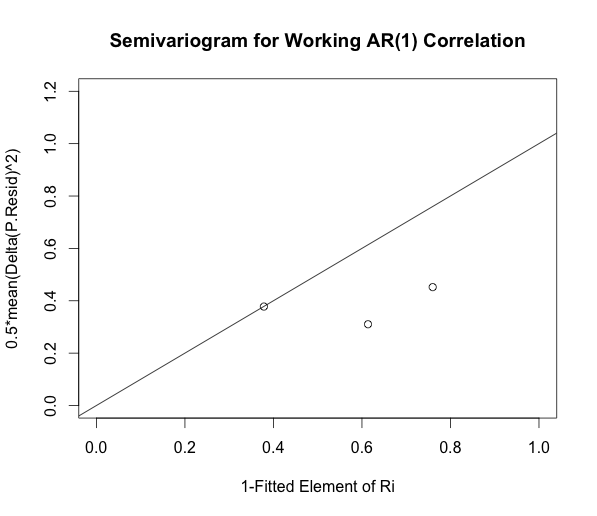
\includegraphics[scale=0.4]{RplotSemiVar.png}		
		\end{figure}
		We fit almost perfectly for the correlation at lag 1, but the fit at higher lags is relatively poor. Perhaps this is due to the fewer number of terms factoring into their computation. The semivariogram for the exchangeable model is not a very complicated plot since there is only a single correlation to estimate. I computed thats estimate in the same way to be $\approx 0.3783865$ compared to the fitted $\widehat\alpha = 0.3899891$. There is nothing really screaming out to me about a violation in any of the assumptions for GEE, so based on all these diagnostics I do not think there is a strong reason to reconsider inference on non-intercept parameters.

	%2
	\item I follow the format of the simulation discussion around slide 50. I set $n=50$ and $B=10^4$ and replicate estimates of $\widehat\beta$ and its estimated standard error. Since we know the data generating mechanism and it's a linear regression of $Y$ on $X$ using independence, we know the true slope $\beta=0.8$. I estimate the true standard error by the sample mean of the estimates from the bootstrap. Histograms from the simulation are  
		\begin{figure}[H]
			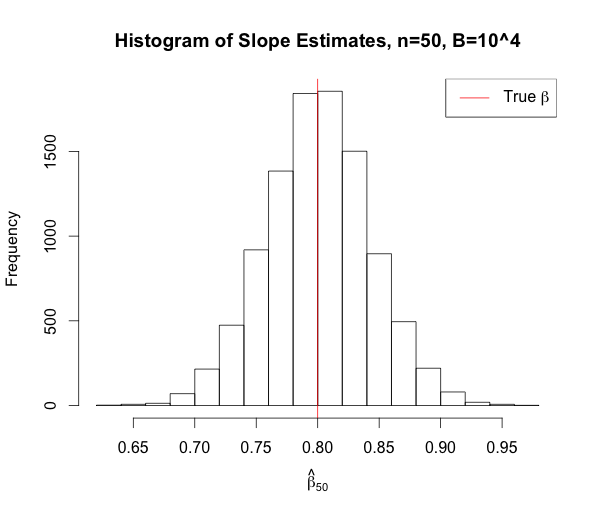
\includegraphics[scale=0.4]{Rplotp21}
			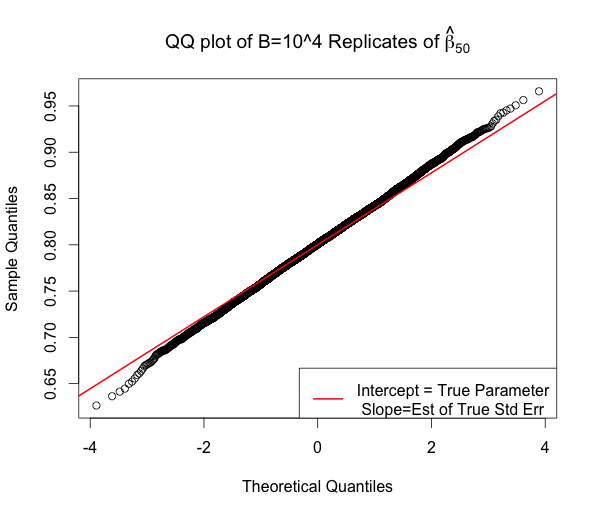
\includegraphics[scale=0.4]{Rplotp22}			
		\end{figure}
		
		\begin{figure}[H]
			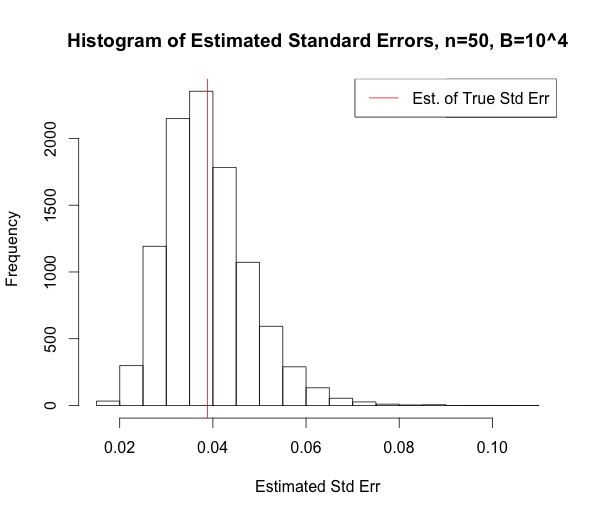
\includegraphics[scale=0.4]{Rplotp23}
			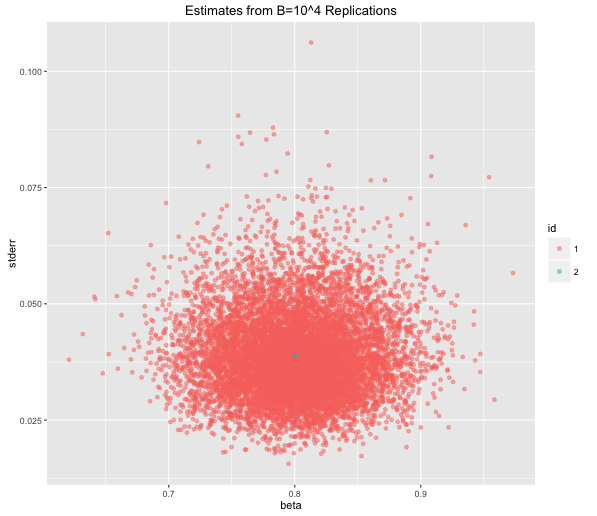
\includegraphics[scale=0.4]{Rplotp24}	
		\end{figure}
		We know increasing $n$ yields nominal coverage, but in this case, it does not look like we had the strong correlation between estimates of the standard error and estimates of the slope, which helps explain why we're losing some coverage at this relatively small $n$. Moreover, we see much smaller variability in the empirical distribution of the standard errors and evident non-normality (which is okay). Unlike the case where large values of $\widehat\beta$ also corresponded to larger standard errors, the fourth scatter plot suggests that standard errors aren't responding in like manner to allow the asymptotics to kick in as early as they would in other examples. There does appear to be a bit of a U shape in the scatter plot, so perhaps we tend to see very large positive and negative values of $(\widehat\beta - 0.8)$ together with extremely large values of standard errors, but this appears infrequently.
	%3
	\item
		\begin{enumerate}
			\item I chose $n=10^4$ clusters for the linear regression of $Y$ on $X$ according to the model in the problem for $\beta_2\in \{-5,-4.5,\dotsc,4.5,5\}$ under both working correlation assumptions. My limiting values against choice of $\beta_2$ are
				\begin{figure}[H]
				\centering
				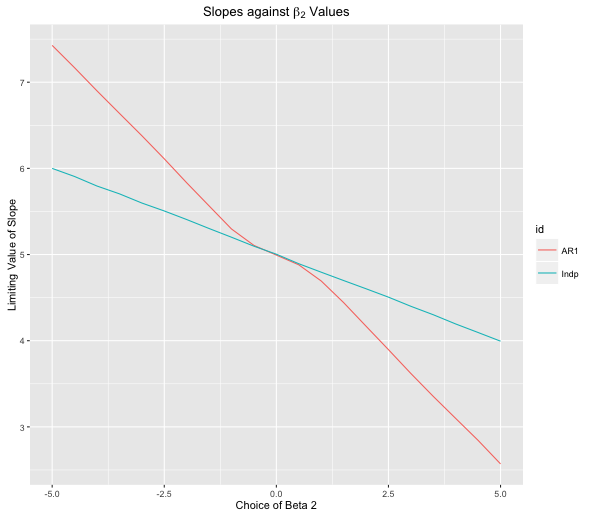
\includegraphics[scale=0.4]{Rplotp41}
				\end{figure}
		In both cases, we have a biased estimate of the true parameter for all choices of $\beta_2\neq 0$. For positive choices of $\beta_2$ we have negative bias and the reverse is true for negative choices of $\beta_2$. The bias is larger for the AR(1) working correlation assumption, and the difference in bias becomes much more pronounced as $\beta_2$ increases in magnitude. The mean model we fit is
		\[
			E[Y_{ij} | X_{ij}=x_{ij}] = \beta_0 + \beta_1^*x_{ij},
		\]
		compared to the data generating mechanism, where the truth is
		\[
			E[Y_{ij}| X_{ij}=x_{ij}] = \mu_{ij} = \beta_1x_{ij} + \beta_2\bm{1}_{x_{ij}=2} - \beta_2 \bm{1}_{x_{ij}=3}.
		\]
		Working this out, the truth says that the conditional mean of any cluster is
		\[
			E[Y_i | X_i] = \begin{pmatrix}
				\beta_1 \\
				2\beta_1 + \beta_2 \\
				3\beta_1 - \beta_2 \\
				4\beta_1
			\end{pmatrix} = \beta_1 \begin{pmatrix}
				1 \\ 2 \\ 3 \\ 4
			\end{pmatrix} + \beta_2 \begin{pmatrix}
				0 \\ 1 \\ -1 \\ 0
			\end{pmatrix}
		\]
		and thus the random vector $Y_i|X_i$ is multivariate normal with that mean and covariance $I_4$. The model we fit tries to realize
		\[
			E[Y_i|X_i] =  \beta_0 \begin{pmatrix}
				1 \\ 1 \\ 1 \\ 1
			\end{pmatrix} + \beta_1^* \begin{pmatrix}
				1 \\ 2 \\ 3 \\ 4
			\end{pmatrix}
		\]
		under both working correlations. For $\beta_2\neq 0$, hoping for $\widehat{\beta_1^*} = \beta_1$ is a lost cause. However, deviations in the estimates $\widehat{\beta_1^*}_{Indp}$ and $\widehat{\beta_1^*}_{AR(1)}$ can be explained by thinking about the weights on observations within a cluster for both working correlations. Obviously for independence, all observations are weighted equally and we have a plain-vanilla OLS with a misspecified mean model. The estimating equations we need to solve are
		\[
			X^T(\sum_{i=1}^n Y_i - X\beta) = \bm{0}_2,
		\]
		where $\bm{X}_i$ does not depend on $i$ so $X^T = \begin{pmatrix}
			1 & 1 & 1 & 1 \\ 1 & 2 & 3 & 4
		\end{pmatrix}$ and obviously $g$ is the identity in the linear regression case. Under the independence working correlation, for very large $n$, we can say we're going to end up solving the system
		\[
			X^T (\overline{\bm{Y}} - X\beta) = \bm{0}_2,
		\]
		where $\overline{\bm{Y}} = \begin{pmatrix}
				\beta_1 \\
				2\beta_1 + \beta_2 \\
				3\beta_1 - \beta_2 \\
				4\beta_1
			\end{pmatrix}$ by the law of large numbers. Writing all this out, for very large $n$ we want $(\beta_0,\beta_1^*)^T$ that solves
			\[
				\begin{pmatrix}
			1 & 1 & 1 & 1 \\ 1 & 2 & 3 & 4
		\end{pmatrix} \left[\begin{pmatrix}
				\beta_1 \\
				2\beta_1 + \beta_2 \\
				3\beta_1 - \beta_2 \\
				4\beta_1
			\end{pmatrix} - \begin{pmatrix}
				\beta_0 + \beta_1^* \\
				\beta_0 + 2\beta_1^* \\
				\beta_0 + 3\beta_1^* \\
				\beta_0 + 4\beta_1^*
			\end{pmatrix} \right].
			\]
			Multiplying this out, this reduces to the linear system of two equations in two unknowns (in the generating model, we know $\beta_2$ and $\beta_1$),
			\begin{align*}
				2\beta_0 + 5\beta_1^* &= 5\beta_1 \\
				-10\beta_0 - 30\beta_1^* &= -30\beta_1 + \beta_2,
			\end{align*}
			which we can solve easily to find asymptotic solutions $\widehat{\beta_0} = \beta_2/2$ and $\widehat{\beta_1^*} = \beta_1-\beta_2/5$.
		When we try an AR(1) working correlation, we are saying that observations in a cluster at lag 1 have stronger correlation than those at lag 2 and even stronger than those at lag 3, and since $S=1$ in this case and since we know $\phi$ does not play a role in the estimation, our new set of estimating equations is asmyptotically
		\[
			X^T V^{-1} (\overline{\bm{Y}} - X\beta) = \bm{0}_2,
		\]	
		where $V^{-1}$ is the inverse of the $4\times 4$ AR(1) working correlation matrix, an inverse we've computed in previous problem sets. I wrote out this system in Mathematica and analytically solved it in terms of the unknown quantity $\alpha$ that GEE also estimates. I appended my Mathematica code, but the answer (asymptotic as usual) is
		\begin{align*}
			\widehat{\beta_0} &= \frac{5\beta_2(1-\alpha)^2}{10-5\alpha+\alpha^2} \\
			\widehat{\beta_1} &= \frac{(10-5\alpha+\alpha^2)\beta_1 - 2(1-\alpha)^2\beta_2}{10-5\alpha+\alpha^2}.
		\end{align*}
		I do not have a great interpretation of these answers except that when $\alpha=0$ we recover the old formula. Roughly, the inverse matrix $V^{-1}$ places weights on observations at closer lags, but observations at closer lags are pretty far apart in the data generating mechanism for $\beta_2\neq 0$ just by looking at the asymptotic conditional mean of a cluster.

		\item The mean model misspecification invalidates our estimate of the theoretical ``bread matrix" from sandwich theory, so we should not expect nominal coverage of the slope parameter in this case. The theoretical bread matrix $\bm{A}$ is the limiting value of the quantity
		\[
			\frac{1}{n}E\left[\pd{D_i^T}{\beta}V_i^{-1}(Y_i-\mu_i) + D_i^T \pd{V_i^{-1}}{\beta}(Y_i-\mu_i) - D_i^TV_i^{-1}D_i\right].
		\]
		In this problem, we know we've misspecified the mean model, so we lose the nice property where the first two terms under the expectation are necessarily zero from our choice and hence our estimate 
		\[
			\widehat{A} = -\frac{1}{n}\sum_i D_i^TV_i^{-1}D_i
		\]
		should not be consistent in general. This inaccuracy carries through to our estimate $\widehat{\Cov}(\widehat{\beta}) = \widehat{A}^{-1}\widehat{B}\widehat{A}^{T-1}/n$ of the covariance, which we saw in the simulations. I believe the general fact about the sandwich estimators is that they are only semi-robust, in that they are not robust to mean model misspecification in general for this reason. I believe there is at least some protection against this when using canonical links like in 570 though.
		\end{enumerate}
\end{enumerate}
\newpage
R Code
\begin{verbatim}
	library(nlme)
library(ggplot2)
library(geeM)
library(reshape2)
data(Orthodont, package="nlme")
d4 <- Orthodont # using shorter names
d4$id <- d4$Subject
d4$male <- d4$Sex=="Male"
glm1 <- glm(distance~I(age-8)*male, data=d4)
X = model.matrix(glm1)


coplot(distance~age|Subject,data=d4,show.given=F,
       col=c(rep("blue",64),rep("magenta",44)),
       xlim=c(8,14),ylim=c(15,32),
       panel=function(x,y,col,...){points(x,y,col=col)
       lines(x,y,col=col)})
# coplot(distance~age|Subject,data=d4,show.given=F,
#        col=c(rep("blue",48),rep("black",4),rep("blue",12),rep("magenta",8),rep("green",4),rep("magenta",32)),
#        xlim=c(8,14),ylim=c(15,32),
#        panel=function(x,y,col,...){points(x,y,col=col)
#          lines(x,y,col=col)})

dist = matrix(d4$distance,nrow=4,ncol=27,byrow=FALSE)
matplot(d4$age[1:4],dist,type="l",col=c(rep("blue",16),rep("magenta",11)),lty=1,
        xlim=c(8,14),xlab="Age", ylab="Distance (mm)", main="Spaghetti Plot Colored by Gender")
#MALE SUBJECT 13
#his start index is
#(13-1)*4+1
#[1] 49
#end is 53

#19 subject, female #3
#73-76

###first bootstrap
B=1000
fbetaBoot <- matrix(0,nrow=B,ncol=4)

d4blind <- d4
d4blind['blind']=rep(seq(1:27),each=4) #just give me the 27 kids
set.seed(1)
wide <- reshape(d4blind,timevar="age",
                idvar=c("Subject","Sex","id","male","blind"),dir="wide")
for(b in 1:B)
{
  vars = sample(1:27,size=27,replace=TRUE) #indices to use in bootstrap GEE
  boot = wide[vars,] #grab those kids from the WIDE data frame
  long = melt(boot,id.vars=c("Subject","Sex","id","male","blind"),
              measure.vars=c("distance.8","distance.10","distance.12","distance.14"))  
  long = long[as.vector(matrix(1:108,nrow=4,byrow=T)),]
  long['age'] = rep(c(8,10,12,14),27)
  long['bootID'] = rep(1:27,each=4) #have to include this otherwise multiple kids
   appearing won't be distinguished in GEE
  gee1temp <- geem(value~I(age-8)*male, id=bootID, data=long, corstr="ar1")
  fbetaBoot[b,] = gee1temp$beta
}

bootDF <- data.frame(as.vector(fbetaBoot),as.factor(rep(1:4,each=1000)))
names(bootDF) <- c("beta","index")

ggplot(bootDF, aes(x=beta,fill=index)) +
  geom_histogram(data=subset(bootDF, index=="1"), binwidth=0.25) +
  geom_histogram(data=subset(bootDF, index=="2"), binwidth=.025) +
  geom_histogram(data=subset(bootDF, index=="3"), binwidth=0.25) +
  geom_histogram(data=subset(bootDF, index=="4"), binwidth=.05) +
  facet_wrap("index", scales="free")


#now do it for Exchangeable...
fbetaBootE<- matrix(0,nrow=B,ncol=4)
for(b in 1:B)
{
  vars = sample(1:27,size=27,replace=TRUE) #indices to use in bootstrap GEE
  boot = wide[vars,] #grab those kids from the WIDE data frame
  long = melt(boot,id.vars=c("Subject","Sex","id","male","blind"),
              measure.vars=c("distance.8","distance.10","distance.12",
              "distance.14"))  
  long = long[as.vector(matrix(1:108,nrow=4,byrow=T)),]
  long['age'] = rep(c(8,10,12,14),27)
  long['bootID'] = rep(1:27,each=4) #have to include this otherwise multiple
   kids appearing won't be distinguished in GEE
  gee1temp <- geem(value~I(age-8)*male, id=bootID, data=long, corstr="exchangeable")
  fbetaBootE[b,] = gee1temp$beta
}

bootDF2 <- data.frame(as.vector(fbetaBootE),as.factor(rep(1:4,each=1000)))
names(bootDF2) <- c("beta","index")

ggplot(bootDF2, aes(x=beta,fill=index)) +
  geom_histogram(data=subset(bootDF2, index=="1"), binwidth=0.25) +
  geom_histogram(data=subset(bootDF2, index=="2"), binwidth=.025) +
  geom_histogram(data=subset(bootDF2, index=="3"), binwidth=0.25) +
  geom_histogram(data=subset(bootDF2, index=="4"), binwidth=.05) +
  facet_wrap("index", scales="free")

#first ar1, diag for diagnostic
gee1 <- geem(distance~I(age-8)*male, id=id, data=d4, corstr="ar1")
phiAR1 <- gee1$phi
betaAR1 <- gee1$beta
d4DiagAR1 = d4
d4DiagAR1['cluster13'] = c(rep("blue",64),rep("magenta",44))
d4DiagAR1['resid'] = phiAR1^(-1/2)*(d4$distance - X%*%betaAR1)
d4DiagAR1['fitted'] = X%*%betaAR1
plot(d4DiagAR1$fitted,d4DiagAR1$resid,xlab="Fitted Values (Distance)",
     ylab="Pearson Residuals", 
     main="Pearson Residuals vs Fitted Values With Lowess iter=0",
     col=d4DiagAR1$cluster13,pch=c(rep(20,48),rep(3,4),rep(20,12),rep(20,8),
     rep(5,4),rep(20,32)))
lines(lowess(fitted.values(gee1),d4DiagAR1$resid,iter=0),col="green")

plot(rep(1:27,each=4),d4DiagAR1$resid,xlab="Child",
     ylab="Pearson Residuals", 
     main="Pearson Residuals vs Cluster Index With Lowess iter=0",
     col=d4DiagAR1$cluster13,pch=c(rep(20,48),rep(3,4),rep(20,12),rep(20,8),
     rep(5,4),rep(20,32)))
lines(lowess(rep(1:27,each=4),d4DiagAR1$resid,iter=0),col="green")


# unitLagAR1 = cbind(d4DiagAR1$resid[-108],d4DiagAR1$resid[-1])
# unitLagAR1 = unitLagAR1[-seq(4,104,4),]
# plot(unitLagAR1)
# abline(a=0,b=gee1$alpha)

plot(d4DiagAR1$fitted,d4DiagAR1$resid^2,xlab="Fitted Values (Distance)",
     ylab="Squared Pearson Residuals", 
     main="Squared P. Residuals vs Fitted Values With Lowess iter=0",
     col=d4DiagAR1$cluster13,
     pch=c(rep(20,48),rep(3,4),rep(20,12),rep(20,8),rep(5,4),rep(20,32)),
     log="y")
lines(lowess(d4DiagAR1$fitted,d4DiagAR1$resid^2,iter=0),col="green")
abline(h=1)

#semivariogram
semialpha1 = matrix(0,nrow=81,ncol=2) 
semialpha2 = matrix(0,nrow=81,ncol=2)
semialpha3 = matrix(0,nrow=81,ncol=2)
count = 1
for(i in seq(1,105,by=4))
{
  semialpha1[count,] = c(d4DiagAR1$resid[i],d4DiagAR1$resid[i+1])
  semialpha1[count+1,] = c(d4DiagAR1$resid[i+1],d4DiagAR1$resid[i+2])
  semialpha1[count+2,] = c(d4DiagAR1$resid[i+2],d4DiagAR1$resid[i+3])
  semialpha2[count,] = c(d4DiagAR1$resid[i],d4DiagAR1$resid[i+2])
  semialpha2[count+1,] = c(d4DiagAR1$resid[i+1],d4DiagAR1$resid[i+3])
  semialpha3[count,] = c(d4DiagAR1$resid[i],d4DiagAR1$resid[i+3])
  count = count + 3
}
semialpha2 = semialpha2[which(rowSums(semialpha2)!=0),]
semialpha3 = semialpha3[which(rowSums(semialpha3)!=0),]


semialpha1Est = 0.5*mean((semialpha1[,1]-semialpha1[,2])^2)
semialpha2Est = 0.5*mean((semialpha2[,1]-semialpha2[,2])^2)
semialpha3Est = 0.5*mean((semialpha3[,1]-semialpha3[,2])^2)

fitted = 1-c(gee1$alpha,gee1$alpha^2,gee1$alpha^3)
plot(fitted,c(semialpha1Est,semialpha2Est,semialpha3Est),xlim=c(0,1),
ylim=c(0,1.2),
     main="Semivariogram for Working AR(1) Correlation",
      xlab="1-Fitted Element of Ri", ylab="0.5*mean(Delta(P.Resid)^2)")
abline(0,1)

#exchangeable
gee2 <- geem(distance~I(age-8)*male, id=id, data=d4, corstr="exchangeable")
phiExch <- gee2$phi
betaExch <- gee2$beta
d4DiagExch = d4
d4DiagExch['cluster13'] = c(rep("blue",64),rep("magenta",44))
d4DiagExch['resid'] = phiExch^(-1/2)*(d4$distance - X%*%betaExch)
d4DiagExch['fitted'] = X%*%betaAR1
plot(d4DiagExch$fitted,d4DiagExch$resid,xlab="Fitted Values (Distance)",
     ylab="Pearson Residuals", 
     main="Pearson Residuals vs Fitted Values With Lowess iter=0",
     col=d4DiagExch$cluster13,pch=c(rep(20,48),rep(3,4),rep(20,12),
     rep(20,8),rep(5,4),rep(20,32)))
lines(lowess(d4DiagExch$fitted,d4DiagExch$resid,iter=0),col="green")

plot(rep(1:27,each=4),d4DiagExch$resid,xlab="Child",
     ylab="Pearson Residuals", 
     main="Pearson Residuals vs Cluster Index With Lowess iter=0",
     col=d4DiagExch$cluster13,pch=c(rep(20,48),rep(3,4),rep(20,12),rep(20,8),
     rep(5,4),rep(20,32)))
lines(lowess(rep(1:27,each=4),d4DiagExch$resid,iter=0),col="green")


unitLagExch = cbind(d4DiagExch$resid[-108],d4DiagExch$resid[-1])
unitLagExch = unitLagExch[-seq(4,104,4),]
0.5*mean((unitLagExch[,1]-unitLagExch[,2])^2)
plot(unitLagExch)
abline(a=0,b=gee2$alpha)




#variance
plot(d4DiagExch$fitted,d4DiagExch$resid^2,xlab="Fitted Values (Distance)",
     ylab="Squared Pearson Residuals", 
     main="Squared P. Residuals vs Fitted Values With Lowess iter=0",
     log="y", col=c(rep("blue",64),rep("magenta",44)),pch=c(rep(20,48),rep(3,4),rep(20,12),rep(20,8),
     rep(5,4),rep(20,32)))
lines(lowess(d4DiagExch$fitted,d4DiagExch$resid^2,iter=0),col="green")
abline(h=1)

#LOO bootstraps
B=1000
beta0 <- matrix(0,nrow=B,ncol=27)
beta1 <- matrix(0,nrow=B,ncol=27)
beta2 <- matrix(0,nrow=B,ncol=27)
beta3 <- matrix(0,nrow=B,ncol=27)
d4blind <- d4
d4blind['blind']=rep(seq(1:27),each=4) #just give me the 27 kids
for(i in 1:27)
{
  start = (i-1)*4+1 #grab the starting index to leave one out
  d4temp <- d4blind[-c(start:(start+3)),] #give me the data frame w/o that kiddo
  wide <- reshape(d4temp,timevar="age",
                  idvar=c("Subject","Sex","id","male","blind"),dir="wide")
  for(b in 1:B)
  {
    vars = sample(1:26,size=26,replace=TRUE) #indices to use in bootstrap GEE
    boot = wide[vars,] #grab those kids from the WIDE data frame
    long = melt(boot,id.vars=c("Subject","Sex","id","male","blind"),
         measure.vars=c("distance.8","distance.10","distance.12","distance.14"))
    long = long[as.vector(matrix(1:104,nrow=4,byrow=T)),]
    long['age'] = rep(c(8,10,12,14),26)
    long['bootID'] = rep(1:26,each=4) 
    #have to include this otherwise multiple kids appearing won't be distinguished in GEE
    gee1temp <- geem(value~I(age-8)*male, id=bootID, data=long, corstr="ar1")
    beta0[b,i] = gee1temp$beta[1]
    beta1[b,i] = gee1temp$beta[2]
    beta2[b,i] = gee1temp$beta[3]
    beta3[b,i] = gee1temp$beta[4]
  }
}


#plot bootstrap histograms for each parameter
beta1LOOdf <- data.frame(as.vector(beta1),as.factor(rep(1:27,each=1000)))
names(beta1LOOdf) <- c("beta1", "leftOut")
ggplot(beta1LOOdf, aes(x=leftOut, y=beta1)) + geom_boxplot() 
+ ggtitle("Deletion Diagnostics for Dental Data AR(1)") + xlab("Child Not Appearing") + ylab(expression(paste("Values of ", hat(beta)[1])))

beta0LOOdf <- data.frame(as.vector(beta0),as.factor(rep(1:27,each=1000)))
names(beta0LOOdf) <- c("beta0", "leftOut")
ggplot(beta0LOOdf, aes(x=leftOut, y=beta0)) + geom_boxplot() 
+ ggtitle("Deletion Diagnostics for Dental Data AR(1)") + xlab("Child Not Appearing") + ylab(expression(paste("Values of ", hat(beta)[0])))

beta2LOOdf <- data.frame(as.vector(beta2),as.factor(rep(1:27,each=1000)))
names(beta2LOOdf) <- c("beta2", "leftOut")
ggplot(beta2LOOdf, aes(x=leftOut, y=beta2)) + geom_boxplot() 
+ ggtitle("Deletion Diagnostics for Dental Data AR(1)") + xlab("Child Not Appearing") + ylab(expression(paste("Values of ", hat(beta)[2])))

beta3LOOdf <- data.frame(as.vector(beta3),as.factor(rep(1:27,each=1000)))
names(beta3LOOdf) <- c("beta3", "leftOut")
ggplot(beta3LOOdf, aes(x=leftOut, y=beta3)) + geom_boxplot() 
+ ggtitle("Deletion Diagnostics for Dental Data AR(1)") + xlab("Child Not Appearing") + ylab(expression(paste("Values of ", hat(beta)[3])))


#use GEE to get intervals with the cluster left out
d4blind <- d4
d4blind['blind']=rep(seq(1:27),each=4) #just give me the 27 kids
betas <- matrix(0,nrow=4,ncol=27)
CIbeta0s <- matrix(0,nrow=2,ncol=27)
CIbeta1s <- matrix(0,nrow=2,ncol=27)
CIbeta2s <- matrix(0,nrow=2,ncol=27)
CIbeta3s <- matrix(0,nrow=2,ncol=27)
for(i in 1:27)
{
  start = (i-1)*4+1 #grab the starting index to leave one out
  d4temp <- d4blind[-c(start:(start+3)),] #give me the data frame w/o that kiddo
  geetemp1 <- geem(distance~I(age-8)*male, id=id, data=d4temp, corstr="ar1")
  betas[,i] = summary(geetemp1)$beta
  CIbeta0s[,i] = summary(geetemp1)$se.robust[1]*1.96*c(-1,1)+betas[1,i]
  CIbeta1s[,i] = summary(geetemp1)$se.robust[2]*1.96*c(-1,1)+betas[2,i]
  CIbeta2s[,i] = summary(geetemp1)$se.robust[3]*1.96*c(-1,1)+betas[3,i]
  CIbeta3s[,i] = summary(geetemp1)$se.robust[4]*1.96*c(-1,1)+betas[4,i]
}
plot(1:27,betas[1,],ylim=c(19,23),col="red",pch=20,
     main="Intercept Estimate, Leaving out Cluster with 95% GEE Interval", xlab="Cluster Omitted", ylab=expression(paste(hat(beta)[0], "with Confidence Interval")))
for(i in 1:27)
{
  segments(x0=i,y0=CIbeta0s[1,i],x1=i,y1=CIbeta0s[2,i])
}
plot(1:27,betas[2,],ylim=c(0.3,0.7),col="red",pch=20,
 main="Slope Estimate, Leaving out Cluster with 95% GEE Interval", xlab="Cluster Omitted", ylab=expression(paste(hat(beta)[1], "with Confidence Interval")))
for(i in 1:27)
{
  segments(x0=i,y0=CIbeta1s[1,i],x1=i,y1=CIbeta1s[2,i])
}
plot(1:27,betas[3,],ylim=c(-0.5,3.5),col="red",pch=20,
     main="Slope Estimate, Leaving out Cluster with 95% GEE Interval", xlab="Cluster Omitted", ylab=expression(paste(hat(beta)[2], "with Confidence Interval")))
for(i in 1:27)
{
  segments(x0=i,y0=CIbeta2s[1,i],x1=i,y1=CIbeta2s[2,i])
}
plot(1:27,betas[4,],col="red",ylim=c(0,0.6),pch=20,
     main="Slope Estimate, Leaving out Cluster with 95% GEE Interval", xlab="Cluster Omitted", ylab=expression(paste(hat(beta)[3], "with Confidence Interval")))
for(i in 1:27)
{
  segments(x0=i,y0=CIbeta3s[1,i],x1=i,y1=CIbeta3s[2,i])
}


####now do all that boot LOO for exchangeable
B=1000
beta0 <- matrix(0,nrow=B,ncol=27)
beta1 <- matrix(0,nrow=B,ncol=27)
beta2 <- matrix(0,nrow=B,ncol=27)
beta3 <- matrix(0,nrow=B,ncol=27)
d4blind <- d4
d4blind['blind']=rep(seq(1:27),each=4) #just give me the 27 kids
set.seed(1)
for(i in 1:27)
{
  start = (i-1)*4+1 #grab the starting index to leave one out
  d4temp <- d4blind[-c(start:(start+3)),] #give me the data frame w/o that kiddo
  wide <- reshape(d4temp,timevar="age",
                  idvar=c("Subject","Sex","id","male","blind"),dir="wide")
  for(b in 1:B)
  {
    vars = sample(1:26,size=26,replace=TRUE) #indices to use in bootstrap GEE
    boot = wide[vars,] #grab those kids from the WIDE data frame
    long = melt(boot,id.vars=c("Subject","Sex",
    "id","male","blind"),
                measure.vars=c("distance.8","distance.10","distance.12","distance.14"))
    long = long[as.vector(matrix(1:104,nrow=4,byrow=T)),]
    long['age'] = rep(c(8,10,12,14),26)
    long['bootID'] = rep(1:26,each=4) 
    #have to include this otherwise multiple kids appearing won't be distinguished in GEE
    gee1temp <- geem(value~I(age-8)*male, id=bootID, data=long, corstr="exchangeable")
    beta0[b,i] = gee1temp$beta[1]
    beta1[b,i] = gee1temp$beta[2]
    beta2[b,i] = gee1temp$beta[3]
    beta3[b,i] = gee1temp$beta[4]
  }
}


#plot bootstrap histograms for each parameter
beta1LOOdf <- data.frame(as.vector(beta1),as.factor(rep(1:27,each=1000)))
names(beta1LOOdf) <- c("beta1", "leftOut")
ggplot(beta1LOOdf, aes(x=leftOut, y=beta1)) + geom_boxplot() 
+ ggtitle("Deletion Diagnostics for Dental Data Exchangeable") + xlab("Child Not Appearing") + ylab(expression(paste("Values of ", hat(beta)[1])))

beta0LOOdf <- data.frame(as.vector(beta0),as.factor(rep(1:27,each=1000)))
names(beta0LOOdf) <- c("beta0", "leftOut")
ggplot(beta0LOOdf, aes(x=leftOut, y=beta0)) + geom_boxplot() 
+ ggtitle("Deletion Diagnostics for Dental Data Exchangeable") + xlab("Child Not Appearing") + ylab(expression(paste("Values of ", hat(beta)[0])))

beta2LOOdf <- data.frame(as.vector(beta2),as.factor(rep(1:27,each=1000)))
names(beta2LOOdf) <- c("beta2", "leftOut")
ggplot(beta2LOOdf, aes(x=leftOut, y=beta2)) + geom_boxplot() 
+ ggtitle("Deletion Diagnostics for Dental Data Exchangeable") + xlab("Child Not Appearing") + ylab(expression(paste("Values of ", hat(beta)[2])))

beta3LOOdf <- data.frame(as.vector(beta3),as.factor(rep(1:27,each=1000)))
names(beta3LOOdf) <- c("beta3", "leftOut")
ggplot(beta3LOOdf, aes(x=leftOut, y=beta3)) + geom_boxplot() 
+ ggtitle("Deletion Diagnostics for Dental Data Exchangeable") + xlab("Child Not Appearing") + ylab(expression(paste("Values of ", hat(beta)[3])))


#use GEE to get intervals with the cluster left out
d4blind <- d4
d4blind['blind']=rep(seq(1:27),each=4) #just give me the 27 kids
betas <- matrix(0,nrow=4,ncol=27)
CIbeta0s <- matrix(0,nrow=2,ncol=27)
CIbeta1s <- matrix(0,nrow=2,ncol=27)
CIbeta2s <- matrix(0,nrow=2,ncol=27)
CIbeta3s <- matrix(0,nrow=2,ncol=27)
for(i in 1:27)
{
  start = (i-1)*4+1 #grab the starting index to leave one out
  d4temp <- d4blind[-c(start:(start+3)),] #give me the data frame w/o that kiddo
  geetemp1 <- geem(distance~I(age-8)*male, id=id, data=d4temp, corstr="exchangeable")
  betas[,i] = summary(geetemp1)$beta
  CIbeta0s[,i] = summary(geetemp1)$se.robust[1]*1.96*c(-1,1)+betas[1,i]
  CIbeta1s[,i] = summary(geetemp1)$se.robust[2]*1.96*c(-1,1)+betas[2,i]
  CIbeta2s[,i] = summary(geetemp1)$se.robust[3]*1.96*c(-1,1)+betas[3,i]
  CIbeta3s[,i] = summary(geetemp1)$se.robust[4]*1.96*c(-1,1)+betas[4,i]
}
plot(1:27,betas[1,],ylim=c(19,23),col="red",pch=20,
     main="Intercept Estimate, Leaving out Cluster with 95% GEE Interval", xlab="Cluster Omitted", ylab=expression(paste(hat(beta)[0], "with Confidence Interval")))
for(i in 1:27)
{
  segments(x0=i,y0=CIbeta0s[1,i],x1=i,y1=CIbeta0s[2,i])
}
plot(1:27,betas[2,],ylim=c(0.3,0.7),col="red",pch=20,
     main="Slope Estimate, Leaving out Cluster with 95% GEE Interval", xlab="Cluster Omitted", ylab=expression(paste(hat(beta)[1], "with Confidence Interval")))
for(i in 1:27)
{
  segments(x0=i,y0=CIbeta1s[1,i],x1=i,y1=CIbeta1s[2,i])
}
plot(1:27,betas[3,],ylim=c(-0.5,3.5),col="red",pch=20,
     main="Slope Estimate, Leaving out Cluster with 95% GEE Interval", xlab="Cluster Omitted", ylab=expression(paste(hat(beta)[2], "with Confidence Interval")))
for(i in 1:27)
{
  segments(x0=i,y0=CIbeta2s[1,i],x1=i,y1=CIbeta2s[2,i])
}
plot(1:27,betas[4,],col="red",ylim=c(0,0.6),pch=20,
     main="Slope Estimate, Leaving out Cluster with 95% GEE Interval", xlab="Cluster Omitted", ylab=expression(paste(hat(beta)[3], "with Confidence Interval")))
for(i in 1:27)
{
  segments(x0=i,y0=CIbeta3s[1,i],x1=i,y1=CIbeta3s[2,i])
}
\end{verbatim}
\newpage
Problem 2
\begin{verbatim}
	library(geeM)
B = 10^4
n = 50
sigma = 1
tau = 1
beta0 = 0
beta1 = 0.8
set.seed(100)
count = 0
ests <- matrix(0,nrow=B,ncol=2)
for(v in 1:B)
{
  nis <- rpois(n,3) + 1
  Z <- matrix(0,nrow=n, ncol=max(nis))
  X <- matrix(0,nrow=n, ncol=max(nis))
  for(i in 1:n)
  {
    for(j in 1:nis[i])
    {
      Z[i,j] = rgamma(1,shape=3,rate=2)
    }
  }
  Z[Z == 0] <- NA
  for(i in 1:n)
  {
    X[i,1:nis[i]] = cumsum(Z[i,1:nis[i]])
  }
  X[X == 0] <- NA
  
  b = rnorm(n,mean=0,sd=tau)
  mu = b + beta0 + beta1*X
  Y <- matrix(0,nrow=n, ncol=max(nis))
  for(i in 1:n)
  {
    for(j in 1:nis[i])
    {
      Y[i,j] = rnorm(1,mean=mu[i,j],sd=sigma)
    }
  }
  Y[Y==0] <- NA
  
  ys = as.vector(t(Y))
  xs = as.vector(t(X))
  simulation = data.frame(ys[!is.na(ys)], xs[!is.na(xs)], rep(1:n,times=nis))
  names(simulation) <- c("y", "x", "id")
  m1 <- geem(y~x, id=id, data=simulation, corstr="independence")
  ci <- 1.96*summary(m1)$se.robust[2]*c(-1,1) + m1$beta[2]
  ests[v,1] = m1$beta[2]
  ests[v,2]=summary(m1)$se.robust[2]
  if(findInterval(beta1,ci) == 1)
  {
    count = count + 1
  }
}
hist(ests[,1],main="Histogram of Slope Estimates, n=50, B=10^4", xlab=expression(hat(beta)[50]))
abline(v=beta1, col="red")
legend("topright",legend=expression(paste("True ", beta)),lty=1,lwd=1,col="red")

estStdErr <- mean(ests[,2])


hist(ests[,2],xlab="Estimated Std Err", main="Histogram of Estimated Standard Errors, n=50, B=10^4")
abline(v=estStdErr, col="red")
legend("topright",legend=expression(paste("Est. of True Std Err")),lty=1,lwd=1,col="red")

plot(qnorm(ppoints(B)),quantile(ests[,1],probs=ppoints(B)),
     main=expression(paste("QQ plot of B=10^4 Replicates of ", hat(beta)[50])),
     xlab="Theoretical Quantiles", ylab="Sample Quantiles")
abline(a=beta1, b=estStdErr,col="red",lwd=2)
legend("bottomright", "Intercept = True Parameter\n Slope=Est of True Std Err",lty=1,lwd=2,col="red")

#plot for joint density
bivariate = data.frame(c(ests[,1],beta1), c(ests[,2],estStdErr),as.factor(rep(c(1,2),times=c(B,1))))
names(bivariate) <- c("beta", "stderr", "id")
ggplot(bivariate, aes(beta, stderr, color=id)) + geom_point(alpha=1/2) + ggtitle("Estimates from B=10^4 Replications")

plot(ests[,1],ests[,2],col="blue")
points(c(beta1,estStdErr),col="red")

# > count
# [1] 9129
\end{verbatim}
\newpage
Problem 3
\begin{verbatim}
	library(ggplot2)
library(gee)
library(geeM)
n = 10000
beta1 = 5
beta2 = seq(-5,5,0.5)
#something in [-5,5]
beta1s <- matrix(0,nrow=1,ncol=length(beta2))
beta1sAR1 <- matrix(0,nrow=1,ncol=length(beta2))

set.seed(1000)
beta2=5
for(k in 1:length(beta2))
{
  X = matrix(rep(1:4,n),nrow=n, ncol=4, byrow=TRUE)
  mu = beta1 * X + beta2[k]*(X==2)-beta2[k]*(X==3)
  Y = matrix(0,nrow=n, ncol=4)
  for(i in 1:n)
  {
    for(j in 1:4)
    {
      Y[i,j] = rnorm(1,mean=mu[i,j], sd=1)
    }
  }
  ys = as.vector(t(Y))
  xs = as.vector(t(X))
  simulations = data.frame(ys,xs,rep(1:n,each=4))
  names(simulations) <- c("y", "x", "id")
  m1 <- geem(y~x, id=id, data=simulations, corstr = "independence")
  beta1s[1,k] = m1$beta[2]
}

#now do it for working cor = AR-1
beta2=5
for(k in 1:length(beta2))
{
  X = matrix(rep(1:4,n),nrow=n, ncol=4, byrow=TRUE)
  mu = beta1 * X + beta2[k]*(X==2)-beta2[k]*(X==3)
  Y = matrix(0,nrow=n, ncol=4)
  for(i in 1:n)
  {
    for(j in 1:4)
    {
      Y[i,j] = rnorm(1,mean=mu[i,j], sd=1)
    }
  }
  ys = as.vector(t(Y))
  xs = as.vector(t(X))
  simulations = data.frame(ys,xs,rep(1:n,each=4))
  names(simulations) <- c("y", "x", "id")
  m1 <- geem(y~x, id=id, data=simulations, corstr = "ar1")
  beta1sAR1[1,k] = m1$beta[2]
}
betaBox <- data.frame(c(beta1s,beta1sAR1),rep(seq(-5,5,0.5),2),as.factor(rep(c("Indp","AR1"),each=length(beta2))))
names(betaBox) <- c("slopes", "true", "id")
ggplot(betaBox, aes(x=true, y=slopes,col=id))  + geom_line() + ggtitle(expression(paste("Slopes against ", beta[2], " Values")))+
  xlab("Choice of Beta 2") + ylab("Limiting Value of Slope")

\end{verbatim}
\end{document}



